\documentclass{article}
\usepackage{blindtext}
\usepackage[a4paper, total={6in, 9.4in}]{geometry}

\usepackage{wrapfig}
\usepackage{graphicx}
\usepackage{mathtext}
\usepackage{amsmath}
\usepackage{siunitx} % Required for alignment
\usepackage{subfigure}
\usepackage{multirow}
\usepackage{rotating}
\usepackage{afterpage}
\usepackage[T1,T2A]{fontenc}
\usepackage[russian]{babel}
\usepackage{caption}
\usepackage[arrowdel]{physics}
\usepackage{booktabs}

\graphicspath{{pictures/}}

\title{\begin{center}Лабораторная работа №3.7.1\end{center}
Скин-эффект в полом цилиндре}
\author{Гёлецян А.Г.}
\date{\today}

\begin{document}

\pagenumbering{gobble}
\maketitle
\newpage
\pagenumbering{arabic}

\textbf{Цель работы:} Исследование проникновения переменного магнитного поля в медный полый цилиндр

\section{Теоретическая часть}
\subsection{Скин-эффект для полупрастранства}
\vspace{1cm}
\begin{wrapfigure}{l}{0.3\textwidth}
  \begin{center}
    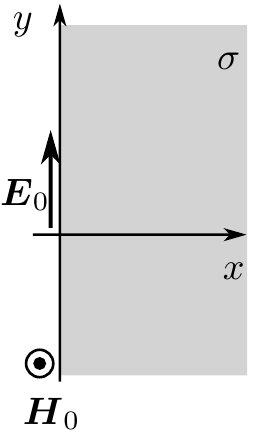
\includegraphics[width=0.28\textwidth]{poluprostranstvo}
  \end{center}
  \caption{Скин-эффект в полупространстве}\label{fig:poluprostranstvo}
\end{wrapfigure}

Рассмотрим квазистационарное поле внутри проводящей среды в простейшем плоском случае.
Пусть вектор $\vb*{E}$ направлен всюду вдоль оси $y$ (рис.\ref{fig:poluprostranstvo}) 
и зависит только от координаты $x$, т. е. ${E_x} = {E_z} \equiv 0$, $E_y=E_y(x,t)$.
В квазистационарном приближении 
\begin{equation*}
    \grad \times \vb*{H} = \sigma \vb*{E}
\end{equation*}
Берем ротор обоих частей
\begin{equation*}
    \grad \times (\grad \times \vb*{H}) = \grad(\grad \cdot \vb*{H}) - \grad^2\vb*{H} = \sigma \grad \times \vb*{E}
\end{equation*}
Испоьзуя ур-е Максвелла для ротора $\vb*{E}$ и для дивергенчии $\vb*{H}$ получаем
\begin{equation}
    \grad^2 \vb*{H} = \sigma\mu\mu_0\frac{\partial\vb*{H}}{\partial t} 
                      + \grad(\grad \cdot \vb*{H}) = \sigma\mu\mu_0\frac{\partial\vb*{H}}{\partial t} 
    \label{eq:laplacian_H}
\end{equation}
Берем ротор еще раз
\begin{equation*}
    \grad \times (\grad^2\vb*{H}) = \grad^2 (\grad \times \vb*{H}) =
    \sigma\mu\mu_0 \frac{\partial (\grad \times \vb*{H})}{\partial t}
\end{equation*}
Осталось подставить первое ур-е, и воспользоватся уравнением Максвелла
\begin{equation}
    \grad^2\vb*{E}=\sigma\mu\mu_0 \frac{\partial \vb*{E}}{\partial t}\label{eq:diffusion}
\end{equation}

Подставляем в (\ref{eq:diffusion}) наше электрическое поле $E_y=E_y(x,t)$
\begin{equation}
    \frac{\partial^2 E_y}{\partial x^2} = \sigma\mu\mu_0\frac{\partial E_y}{\partial t}
    \label{eq:diffusion_chastni}
\end{equation}
Если $E_y(0,t)=E_0 e^{i\omega t}$ то решением (\ref{eq:diffusion_chastni}) будет функция вида
\begin{equation}
    E_y(x,t)=E_0 e^{-x/\delta} e^{i(\omega t - x/\delta)}
    \label{eq:skin_effect_poluprostranstvo}
\end{equation}
где
\begin{equation}
    \delta = \sqrt{\frac{2}{\omega\sigma\mu\mu_0}}
    \label{eq:delta}
\end{equation}

\newpage
\subsection{Скин-эффект в тонокм полом цилиндре}
\vspace{1cm}
\begin{wrapfigure}[36]{l}{0.3\textwidth}
  \begin{center}
    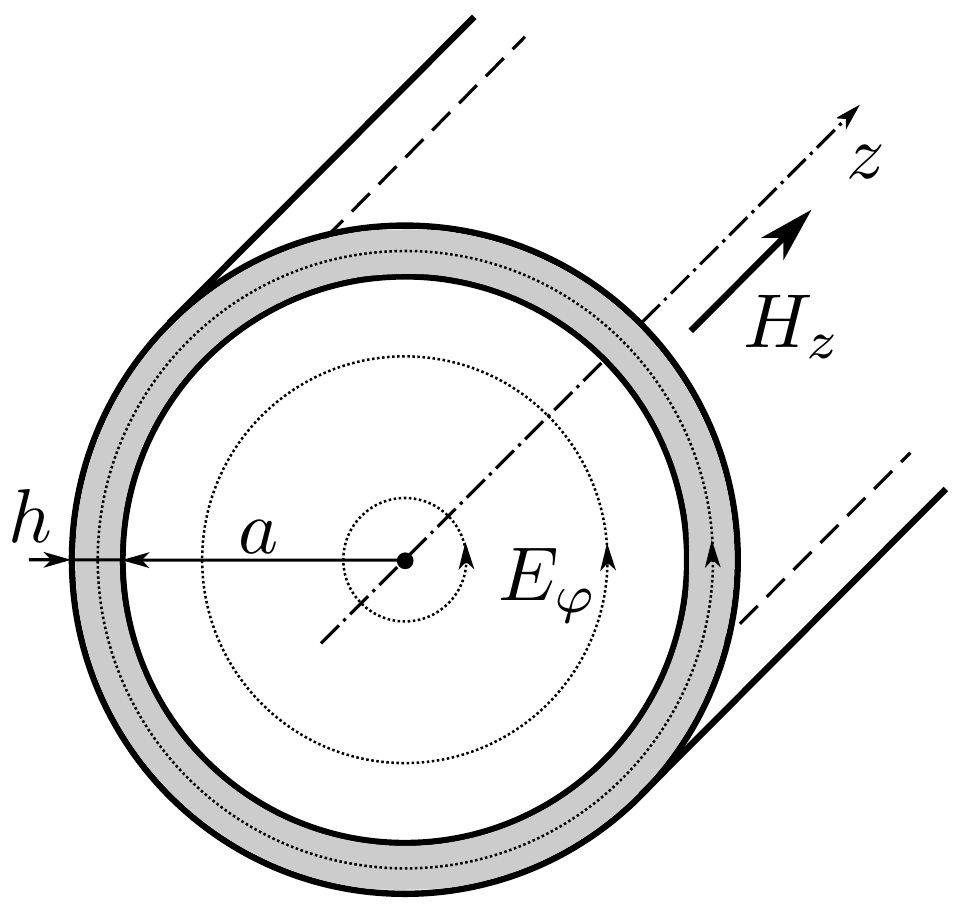
\includegraphics[width=0.28\textwidth]{cilindr}
  \end{center}
  \caption{Эл-магнитные поля в цилиндре}\label{fig:cilindr}

  \begin{center}
    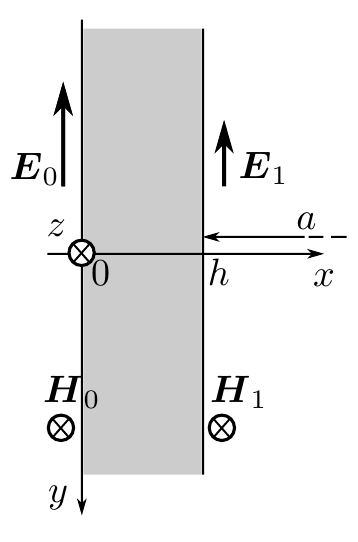
\includegraphics[width=0.28\textwidth]{stenka}
  \end{center}
  \caption{Стенка цилиндра}\label{fig:stenka}
\end{wrapfigure}

Перейдем теперь к описанию теории в нашей работе. Из соображении симметрии и 
непрерывности соответствующих компонет векторов $\vb*{E}$ и $\vb*{H}$ можем сказать что
\begin{equation*}
    H_z = H(r)e^{i\omega t} \text{, } E_\varphi = E(r)e^{i\omega t}
\end{equation*}
и при этом функции $H(r)$ и $E(r)$ непрерывны.

Внутри цилиндра токов нет, следовательно $H(r)=H_1=\text{const}$ внутри цилиндра.
По теореме об электромагнитной индукции
\begin{equation*}
    E(r) = -\frac{1}{2}\mu_0 r \cdot i \omega H_1
\end{equation*}
откуда мы получаем граничное условие
\begin{equation}
    E_1=E(a)= -\frac{1}{2}\mu_0 a \cdot i \omega H_1
    \label{eq:granichnoe_uslovie_E}
\end{equation}

В прближении $h \ll a$ можем пренебречь кривизной стенки и смоделировать 
его бесконечной полосой. Тогда, надо решить уравнение (\ref{eq:laplacian_H})
с граничными условиями. Решая уравнение получим связь полей $H_1$ 
(поле внутри цилиндра которое мы будем измерять) и $H_2$, которое колебается с частотой
$\omega$

\begin{equation}
    H_1 = \frac{H_0}{\ch(\alpha h) + \frac{1}{2} \alpha a \sh(\alpha h)} 
    \text{\ \ \ }
    \alpha = \sqrt{i\omega \sigma \mu_0} = \frac{\sqrt{2}}{\delta}e^{i\pi/4}
    \label{eq:svyaz_poley}
\end{equation}

из этой формулы получим сколько по фазе отстает поле $H_1$ от $H_0$. При $\delta \ll h$
(высокачастотная область)

\begin{equation}
    \psi \approx \frac{\pi}{4} + \frac{h}{\delta} = 
    \frac{\pi}{4} + h \sqrt{\frac{\omega \sigma \mu_0}{2}}
    \label{eq:faza_high_freq}
\end{equation}

При $\delta \gg h$ (низкочастотная область)

\begin{equation}
    \tan \psi \approx \frac{ah}{\delta^2} = \pi a h \sigma \mu \mu_0 \nu
    \label{eq:faza_low_freq}
\end{equation}
\newpage

\subsection{Процесс измерения}
\begin{wrapfigure}{l}{0.5\textwidth}
  \begin{center}
    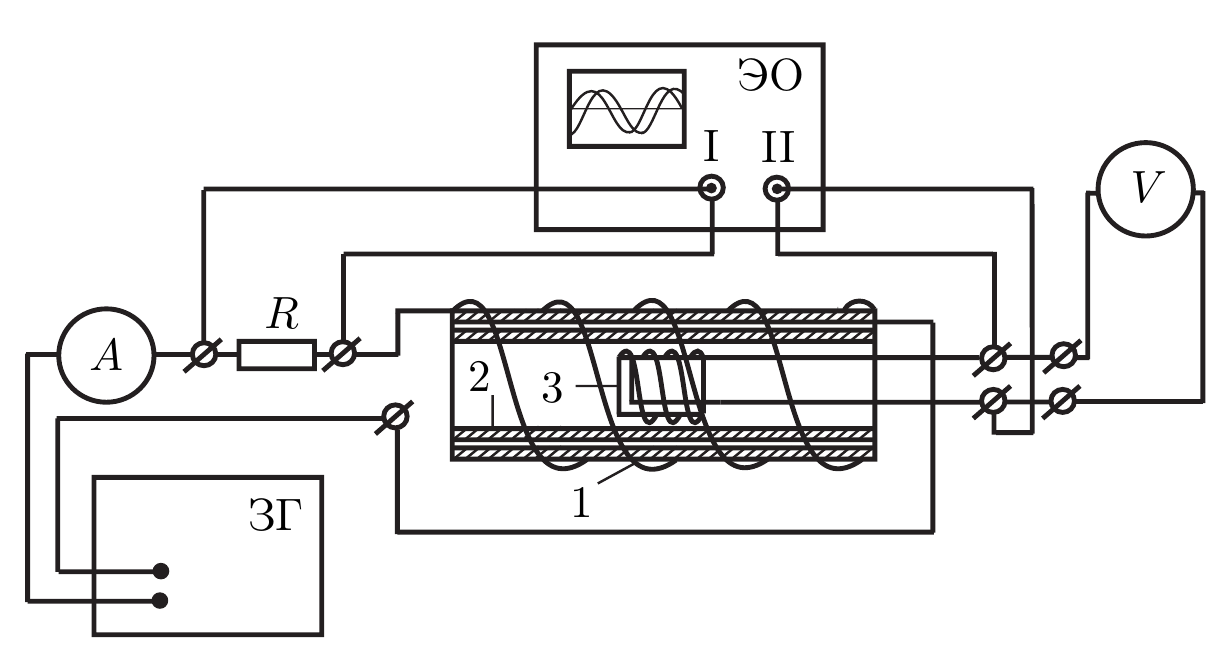
\includegraphics[width=0.48\textwidth]{ustanovka}
  \end{center}
  \caption{Установка}\label{fig:ustanovka}
\end{wrapfigure}

Мангнитное поле внутри цилиндра измеряется катушкой 3. Напряжение на катушке
пропорционалньна производной $\dot{B_1}(t)$
\begin{equation*}
    U(t) \propto \dot{B_1}(t) = -i\omega H_1 e^{i\omega t}
\end{equation*}
Поле внутри цилиндра пропорциональна току через соленоид
\begin{equation*}
    B_0(t) \propto I(t)
\end{equation*}
Отсюда несложно увидеть, что
\begin{equation}
    \frac{\abs{H_1}}{\abs{H_0}} = c \cdot \frac{U}{\nu I} = c \xi
    \label{eq:otnoshenie_amplitud}
\end{equation}
\vspace{0.3cm}

где константу можно определить из условия $\abs{H_1}/\abs{H_2} \rightarrow 1$ при
$\nu \rightarrow 0$.

\vspace{0.3cm}

При измерениях разности фаз нужно учесть, что первый сигнал на осциллографе
пропорционален магнитному полю снаружи, а второй пропорционален производному
поля внутри цилиндра по времени. Вследствии этого набегает дополнительная фаза $\pi/2$,
которую надо вычесть при измерениях.

\newpage
\section{Ход работы}

Параметры нашей установки $2a = 45мм$, $h=1.5мм$. Проводимость порядка
$\sigma \sim 5\cdot 10^7 См/м$. Получаем оценку для частоты, при которой
глубина проникновения равна толщине стенок цилиндра $\nu_h = 2250 Гц$.

\subsection{Измерение проводимости через отношение амплитуд}
В области частот $\nu \ll \nu_h$ $\alpha h \ll 1$, и из (\ref{eq:svyaz_poley}) получаем
\begin{equation*}
    {(c\xi)}^2 \approx \frac{1}{1+A\nu^2}
\end{equation*}
или, эквивалентно
\begin{equation*}
    \frac{1}{\xi^2}=B\nu^2 + c^2 \text{ где } B=\pi a h \sigma \mu_0 c
    \label{eq:liniya_dlya_c}
\end{equation*}

\begin{figure}[h]
    \center{\includegraphics[width=\textwidth]{xi_nu_low_freq_linearized.eps}}
    \caption{График зависимости $1/\xi^2(\nu)$}\label{fig:xi_nu_low_freq_linearized}
    \newpage
\end{figure}

Из графика получаем значение $c$, а так же проводимость меди $\sigma$
\begin{equation}
    c=(72.237 \pm 0.023) \text{, } \sigma = (4.4122 \pm 0.0061) \cdot 10^7 См/м
\end{equation}

\newpage

\subsection{Измерение проводимости через разность фаз в низкочастотном диапазоне}
Согласно формуле (\ref{eq:faza_low_freq}), при $\delta \gg h$
\begin{equation*}
    \tan \psi = k \cdot \nu \ \text{; } k = \pi a h \sigma \mu_0 \ \ (\mu = 1)
\end{equation*}

\begin{figure}[h]
    \center{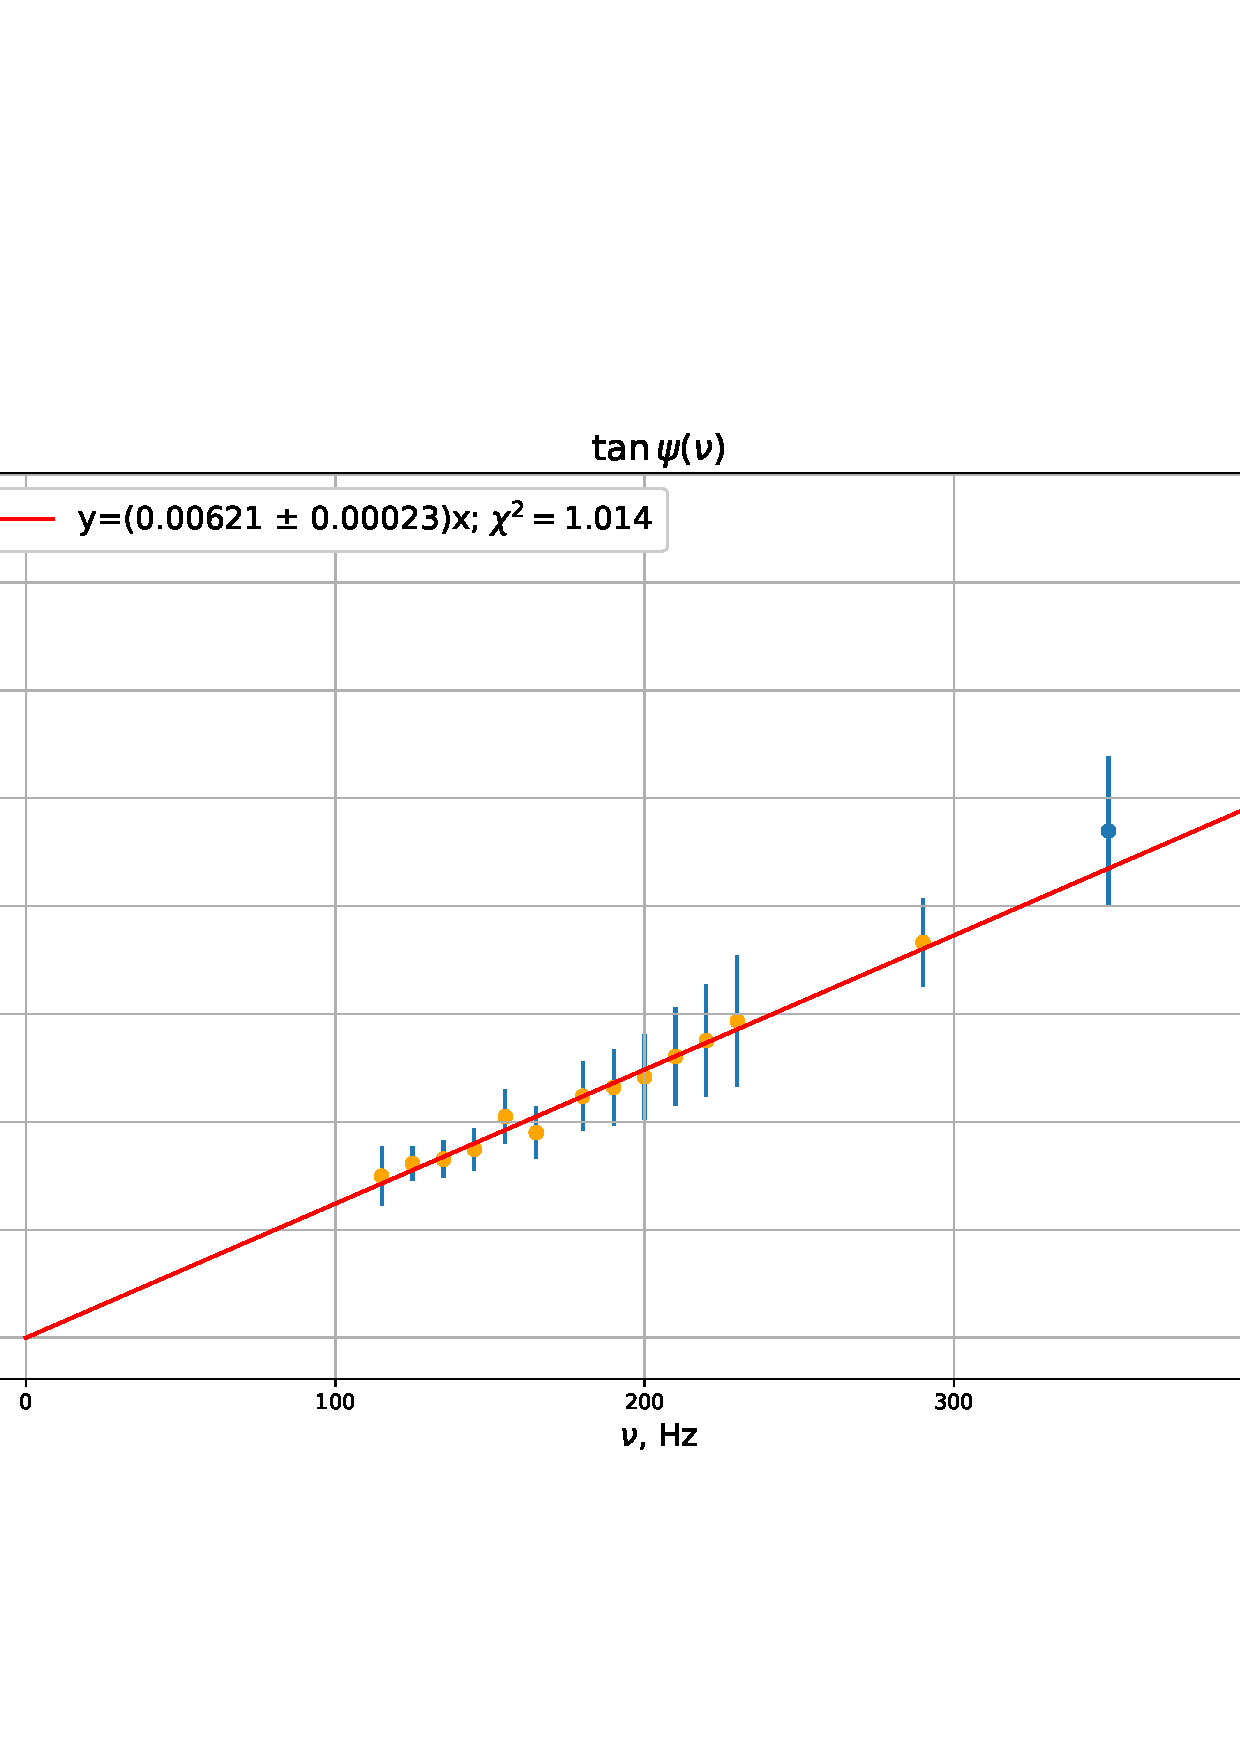
\includegraphics[width=\textwidth]{tg_psi_nu_line}}
    \caption{График зависимости $\tan \psi (\nu)$ (линейная часть)}\label{fig:tg_psi_nu_line}
    \newpage
\end{figure}

\vspace{1cm}
Из коэффициента наклона прямой находим проводимость
\begin{equation}
    \sigma = (4.66 \pm 0.17) \cdot 10^7 См/м
\end{equation}

\newpage

\begin{figure}[h]
    \center{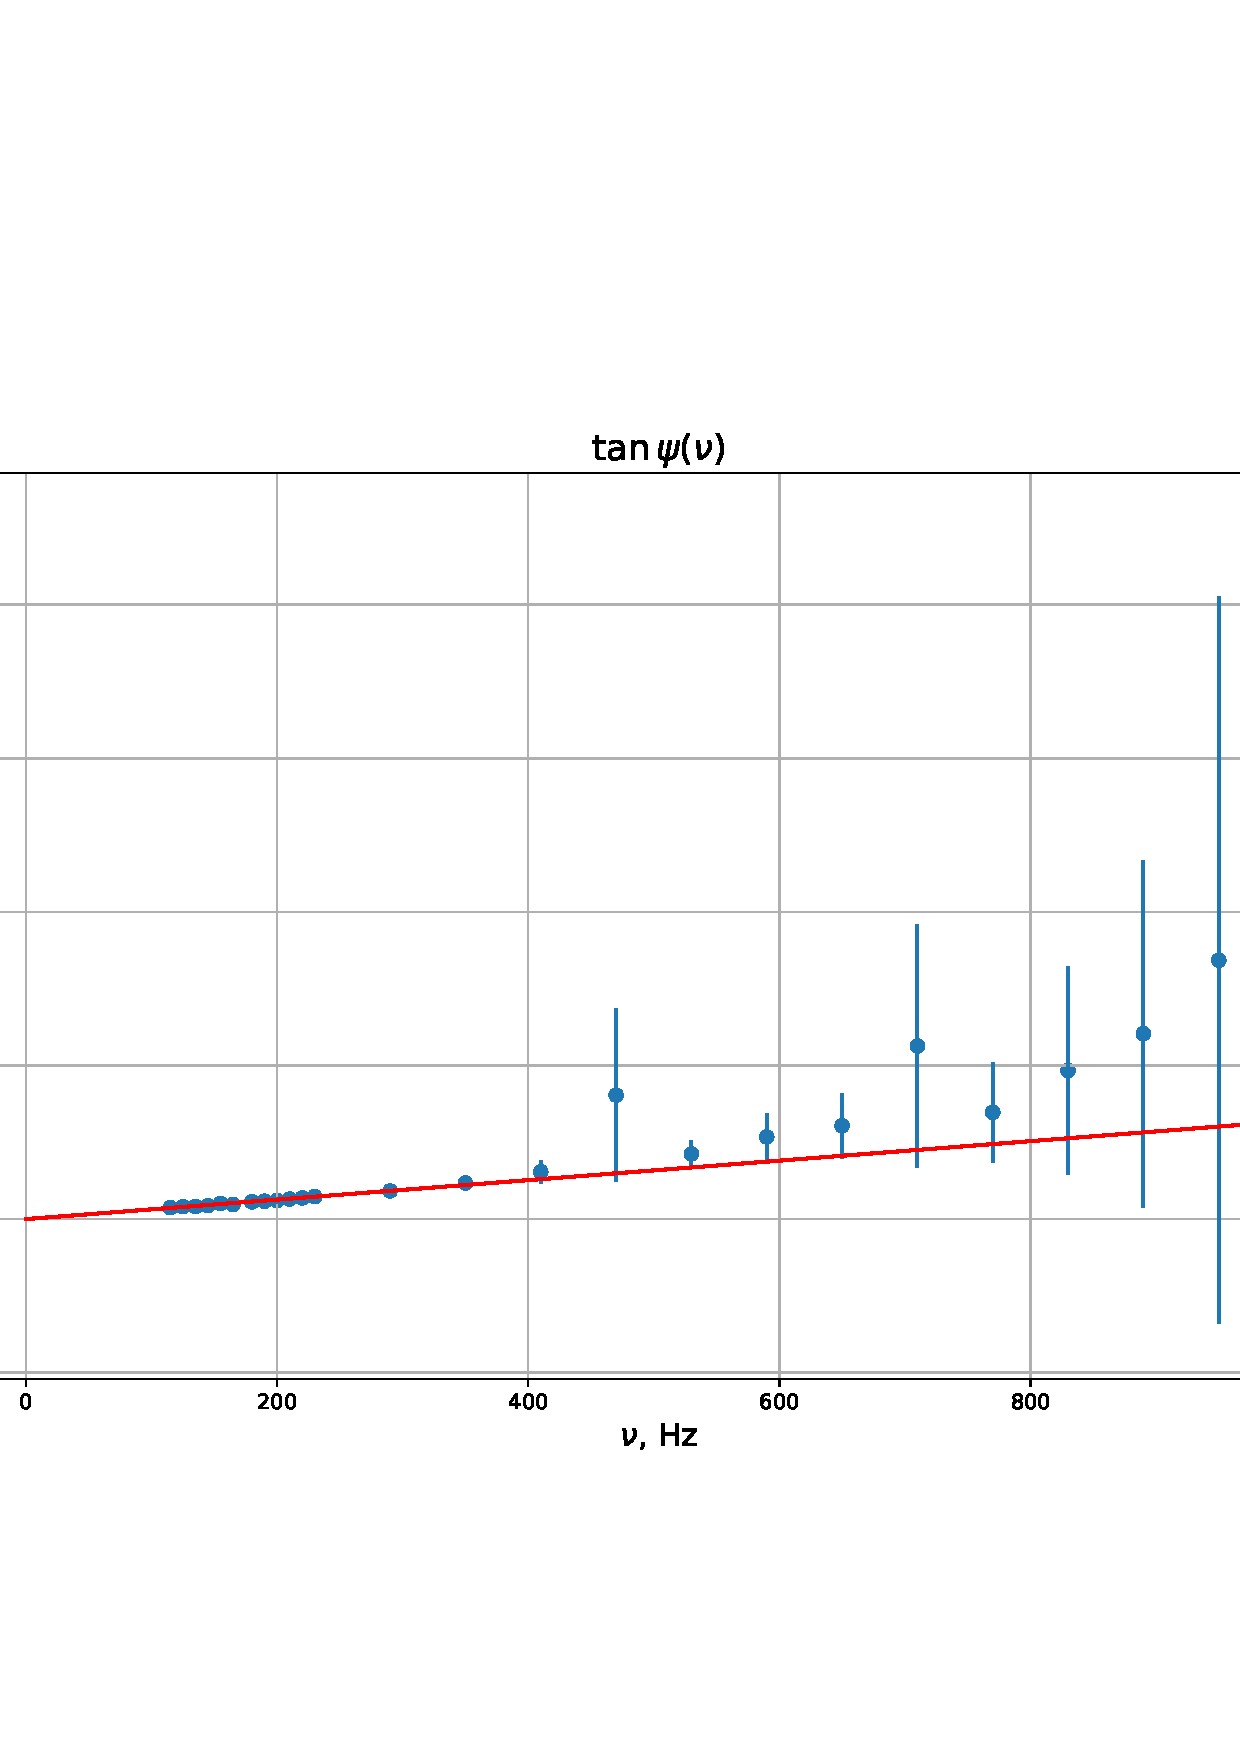
\includegraphics[width=\textwidth]{tg_psi_nu_no_line}}
    \caption{График зависимости $\tan \psi (\nu)$ (нелинейная часть)}\label{fig:tg_psi_nu_no_line}
    \newpage
\end{figure}

\subsection{Измерение проводимости через разность фаз в высокачастотном диапазоне}
Согласно формуле (\ref{eq:faza_high_freq}), при $\delta \ll h$
\begin{equation*}
    \psi - \pi/4 = k\cdot \sqrt{\nu}; \ k = h\sqrt{\pi\mu_0\sigma}
\end{equation*}

Из графика получаем следующее значение проводимости

\begin{equation}
    \sigma = (4.28 \pm 0.33) \cdot 10^7 См/м
\end{equation}

\newpage

\begin{figure}[h]
    \center{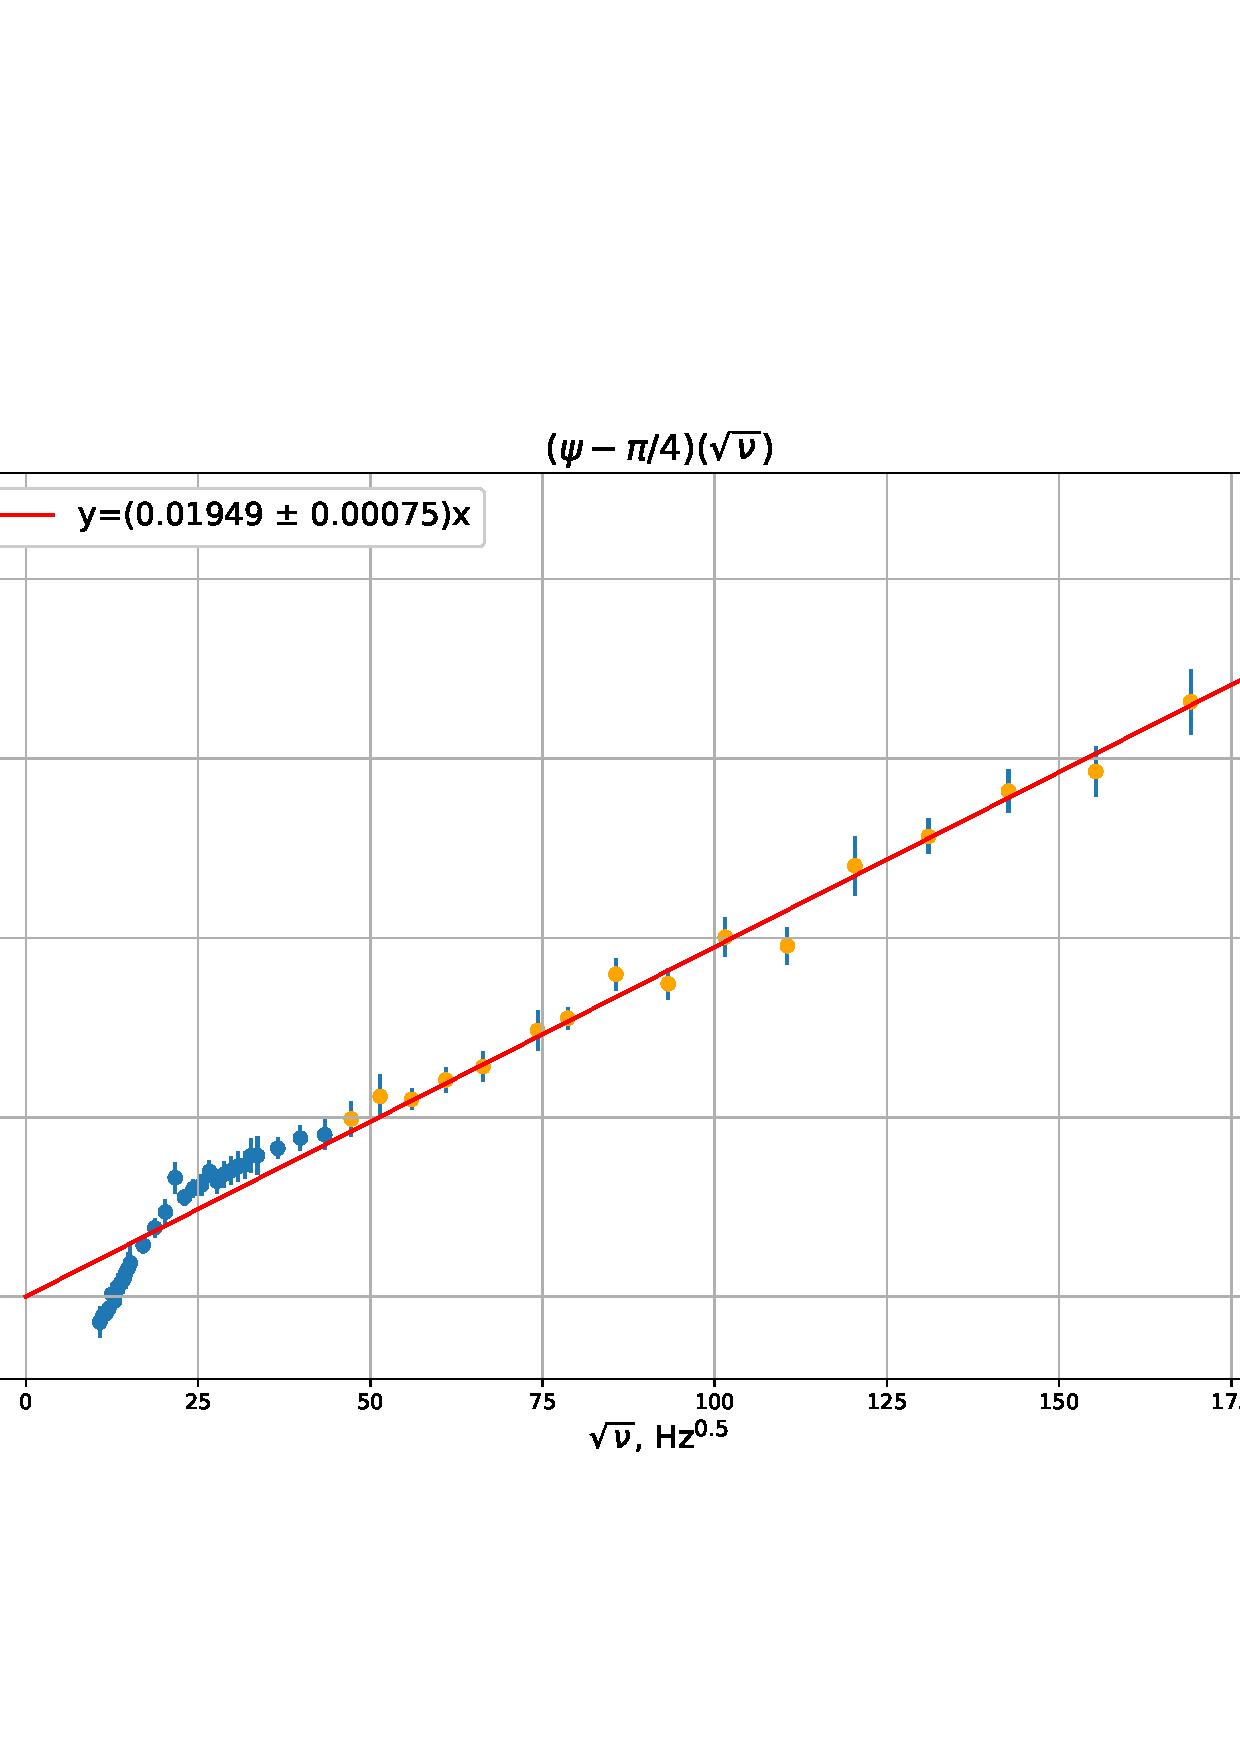
\includegraphics[width=0.9\textwidth]{psi_sqrt_nu}}
    \caption{График зависимости $(\psi - \pi/4)(\sqrt{\nu})$}\label{fig:psi_sqrt_nu}
    \newpage
\end{figure}

\subsection{Измерение проводимости через изменение индуктивности}

Из за наличия цилиндра внутри, индуктивность внешней катушки зависит от катушки
следующим образом

\begin{equation*}
    \frac{L_{\max} - L}{L - L_{\min}} = \pi ^2 a^2 h^2 {\mu_0}^2 \sigma^2 \nu^2
\end{equation*}

\begin{figure}[h]
    \center{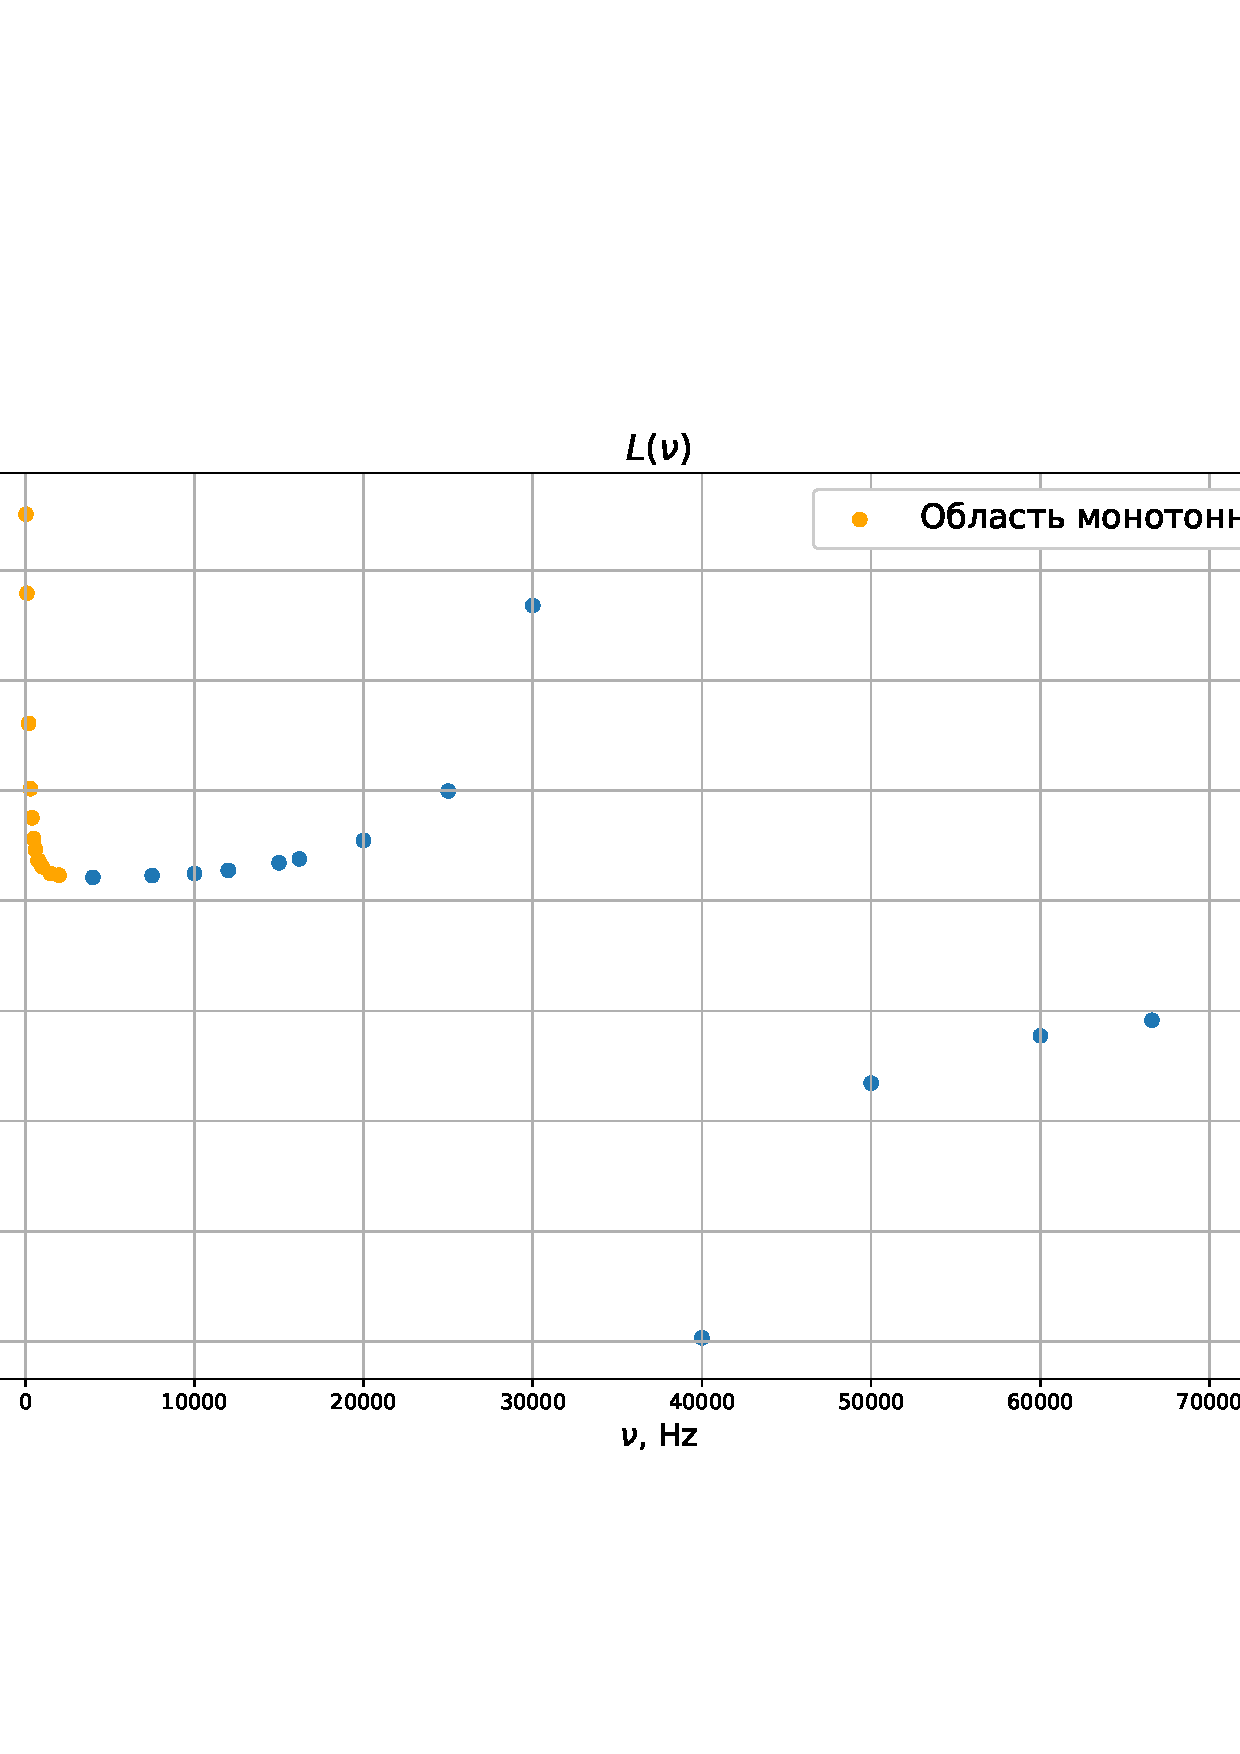
\includegraphics[width=0.7\textwidth]{L_nu}}
    \caption{График зависимости $L(\nu)$}\label{fig:L_nu}
    \newpage
\end{figure}

\newpage

\begin{figure}[h]
    \center{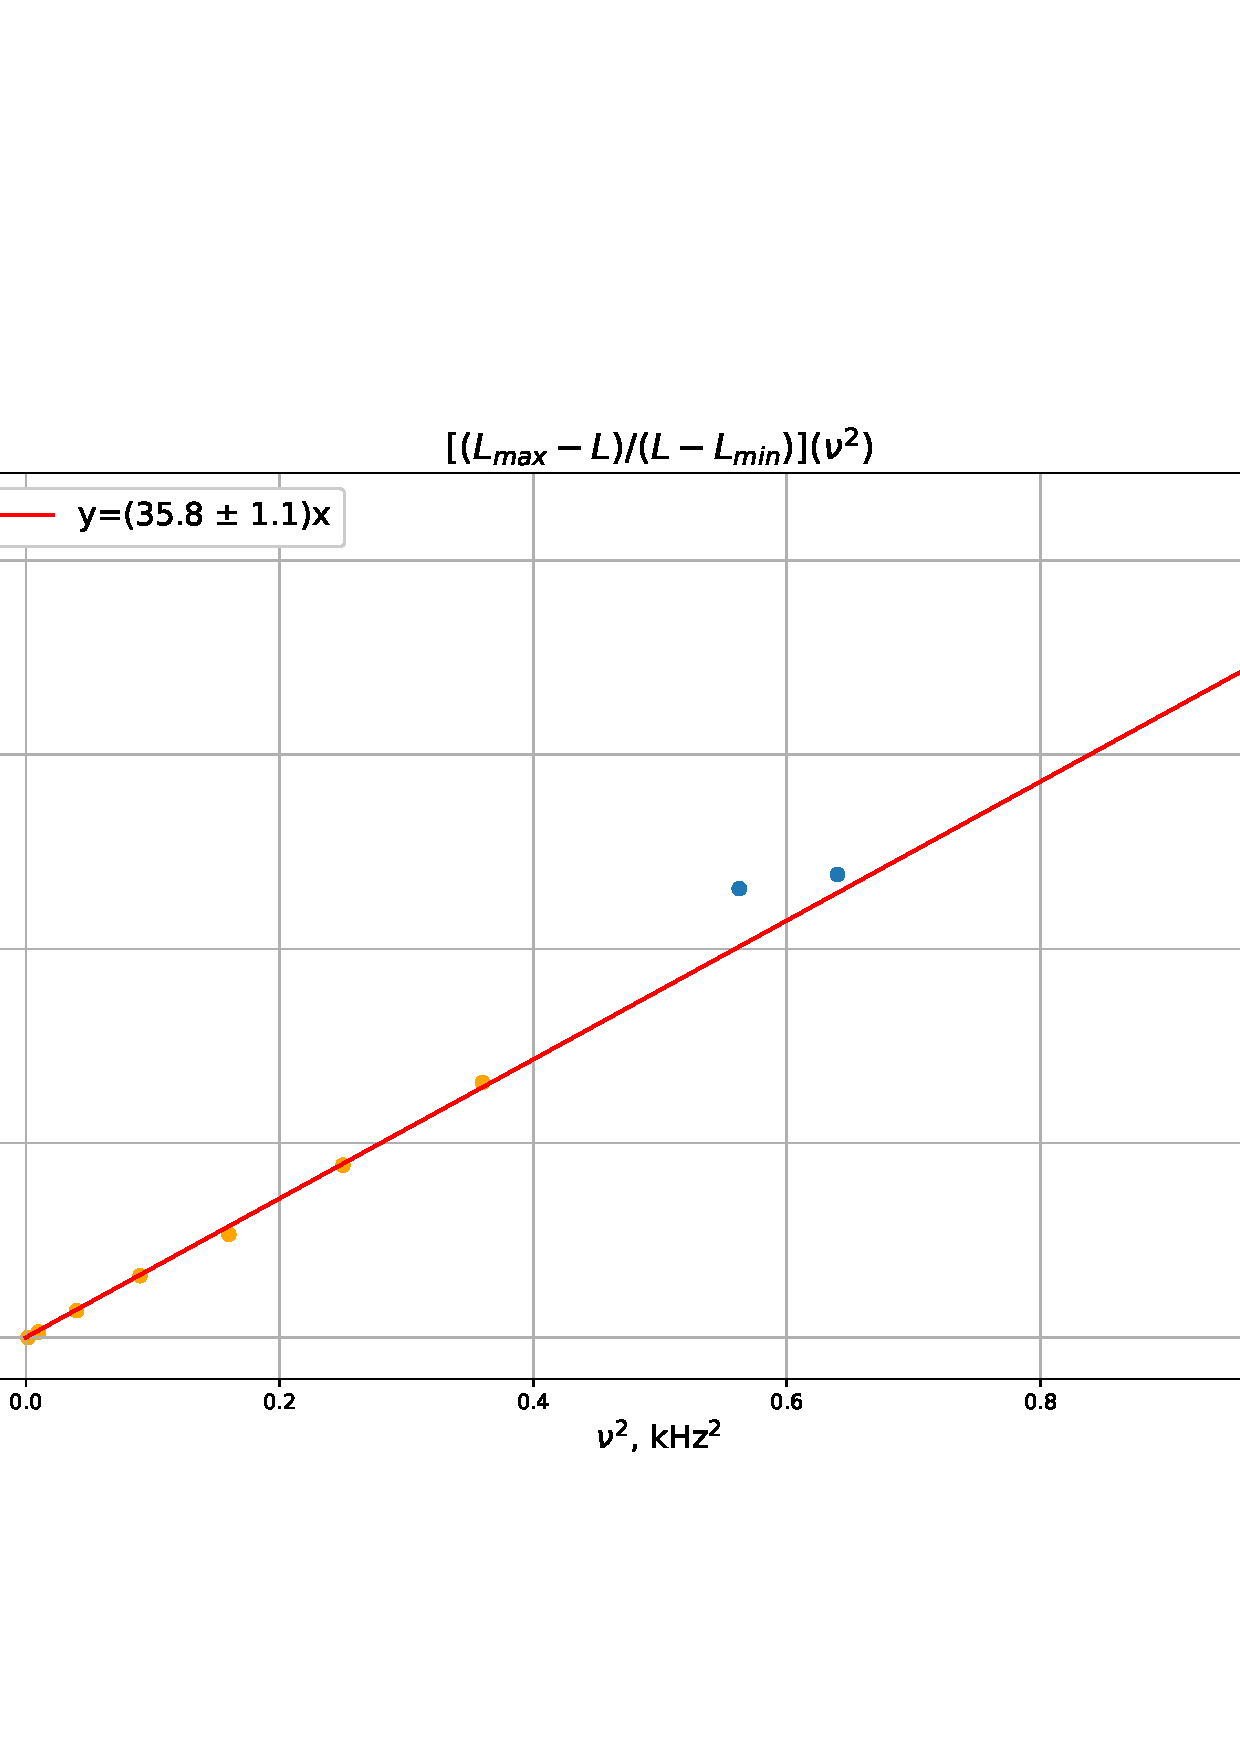
\includegraphics[width=\textwidth]{L_nu_linearized}}
    \caption{График зависимости $\frac{L_{\max} - L}{L - L_{\min}} (\nu^2)$}\label{fig:L_nu_linearized}
    \newpage
\end{figure}

\vspace{1cm}
$L_{\max}$ и $L_{\min}$ ищем в области монотонности. Далее, линеаризуя данные по формуле
выше получаем линейную зависимость при малых $\nu$. По наклону кривой находим

\begin{equation}
    \sigma = (4.49 \pm 0.07) \cdot 10^7 См/м
\end{equation}

\newpage

\subsection{Отношение магнитных полей}
Отношение $\abs{H_1}/\abs{H_0}$ можем посчитать двумя способами. Первый способ - через
формулу (\ref{eq:otnoshenie_amplitud}),использовав значение $c$ из пункта (2.1).
Второй способ - через теоретическую формулу (\ref{eq:svyaz_poley}), использовав значение
$\sigma$ из пункта (2.1). Посмотрим на их различие с помощью графиков зависимости
$\abs{H_1}/\abs{H_0} (\nu)$

\begin{figure}[h]
    \center{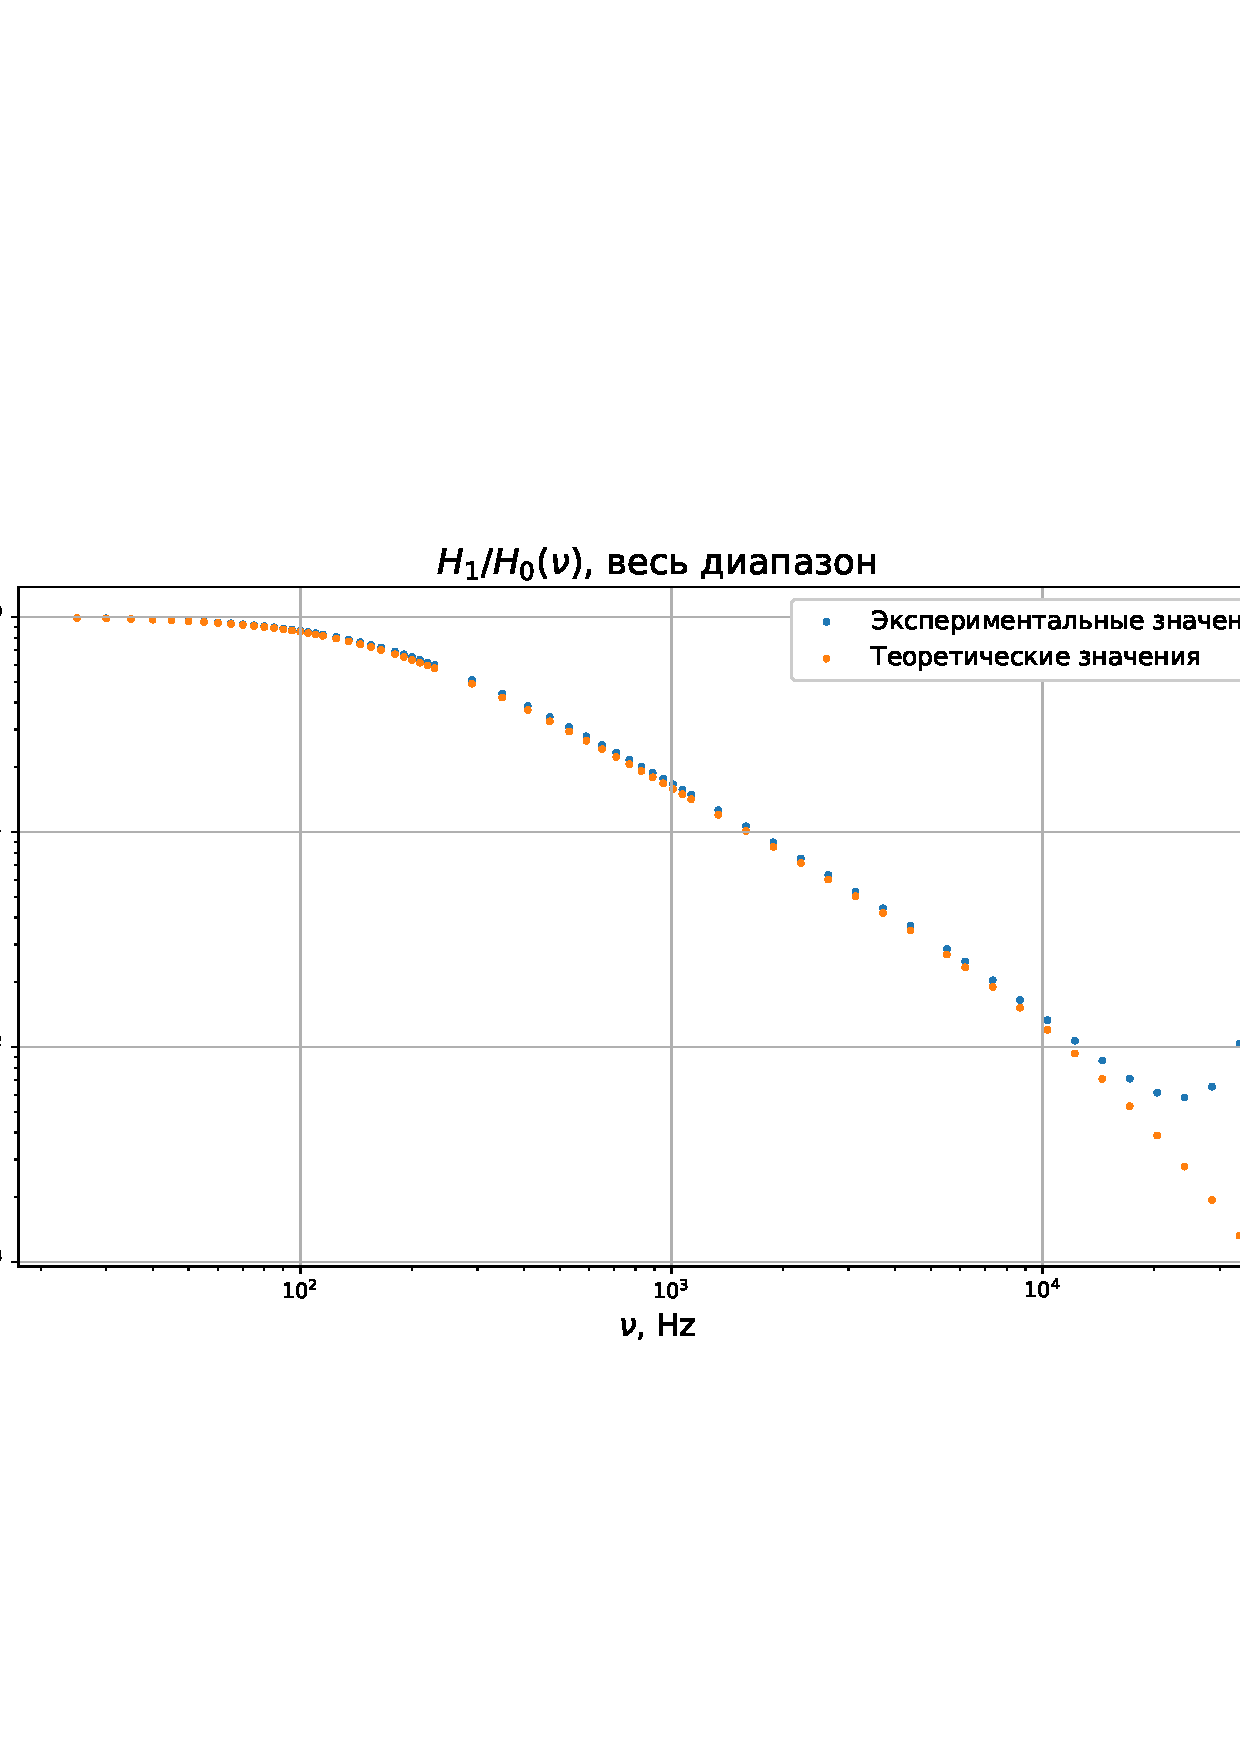
\includegraphics[width=\textwidth]{all_freq_ratio}}
    \caption{Отношение полей - весь диапазон}\label{fig:all_freq_ratio}
    \center{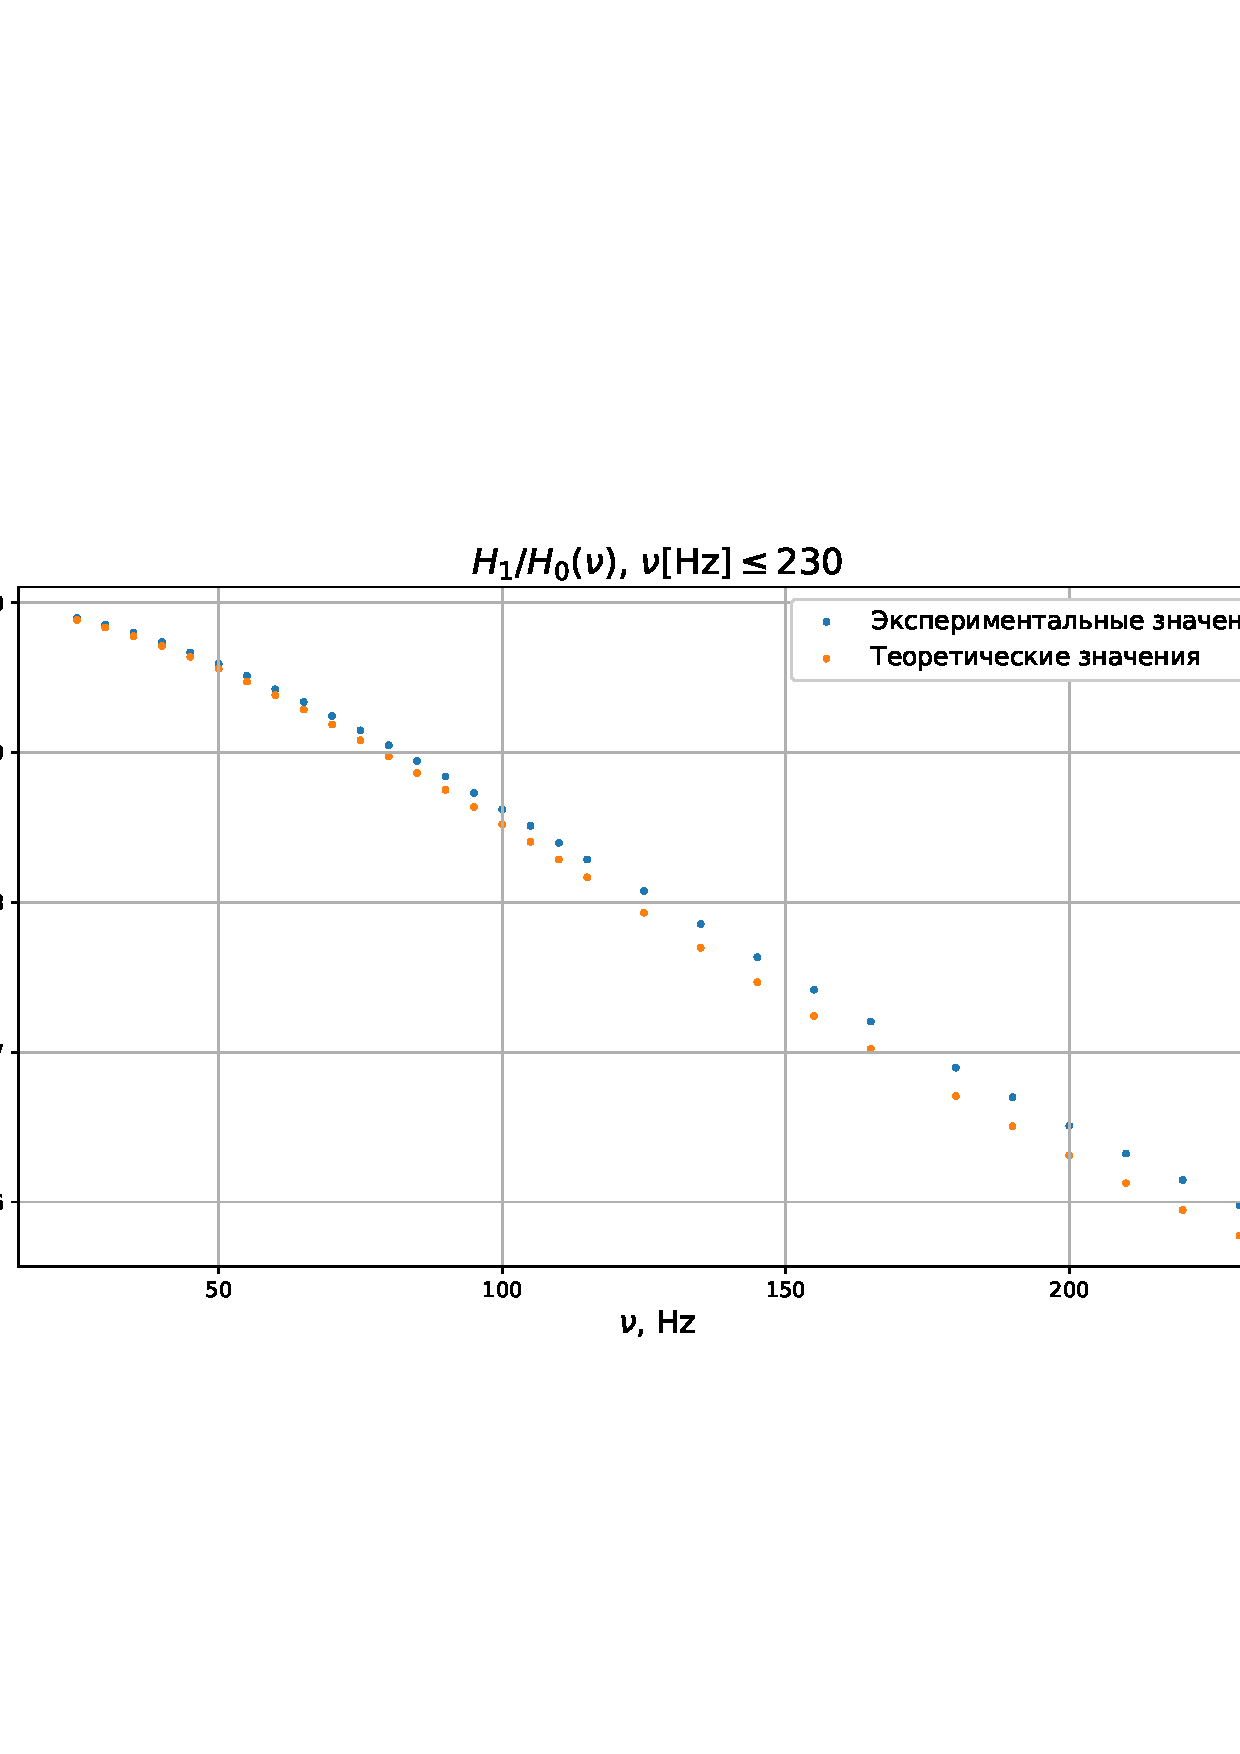
\includegraphics[width=\textwidth]{low_freq_ratio}}
    \caption{Отношение полей - низкочастотный диапазон}\label{fig:low_freq_ratio}
    \newpage
\end{figure}

\newpage

\begin{figure}[h]
    \center{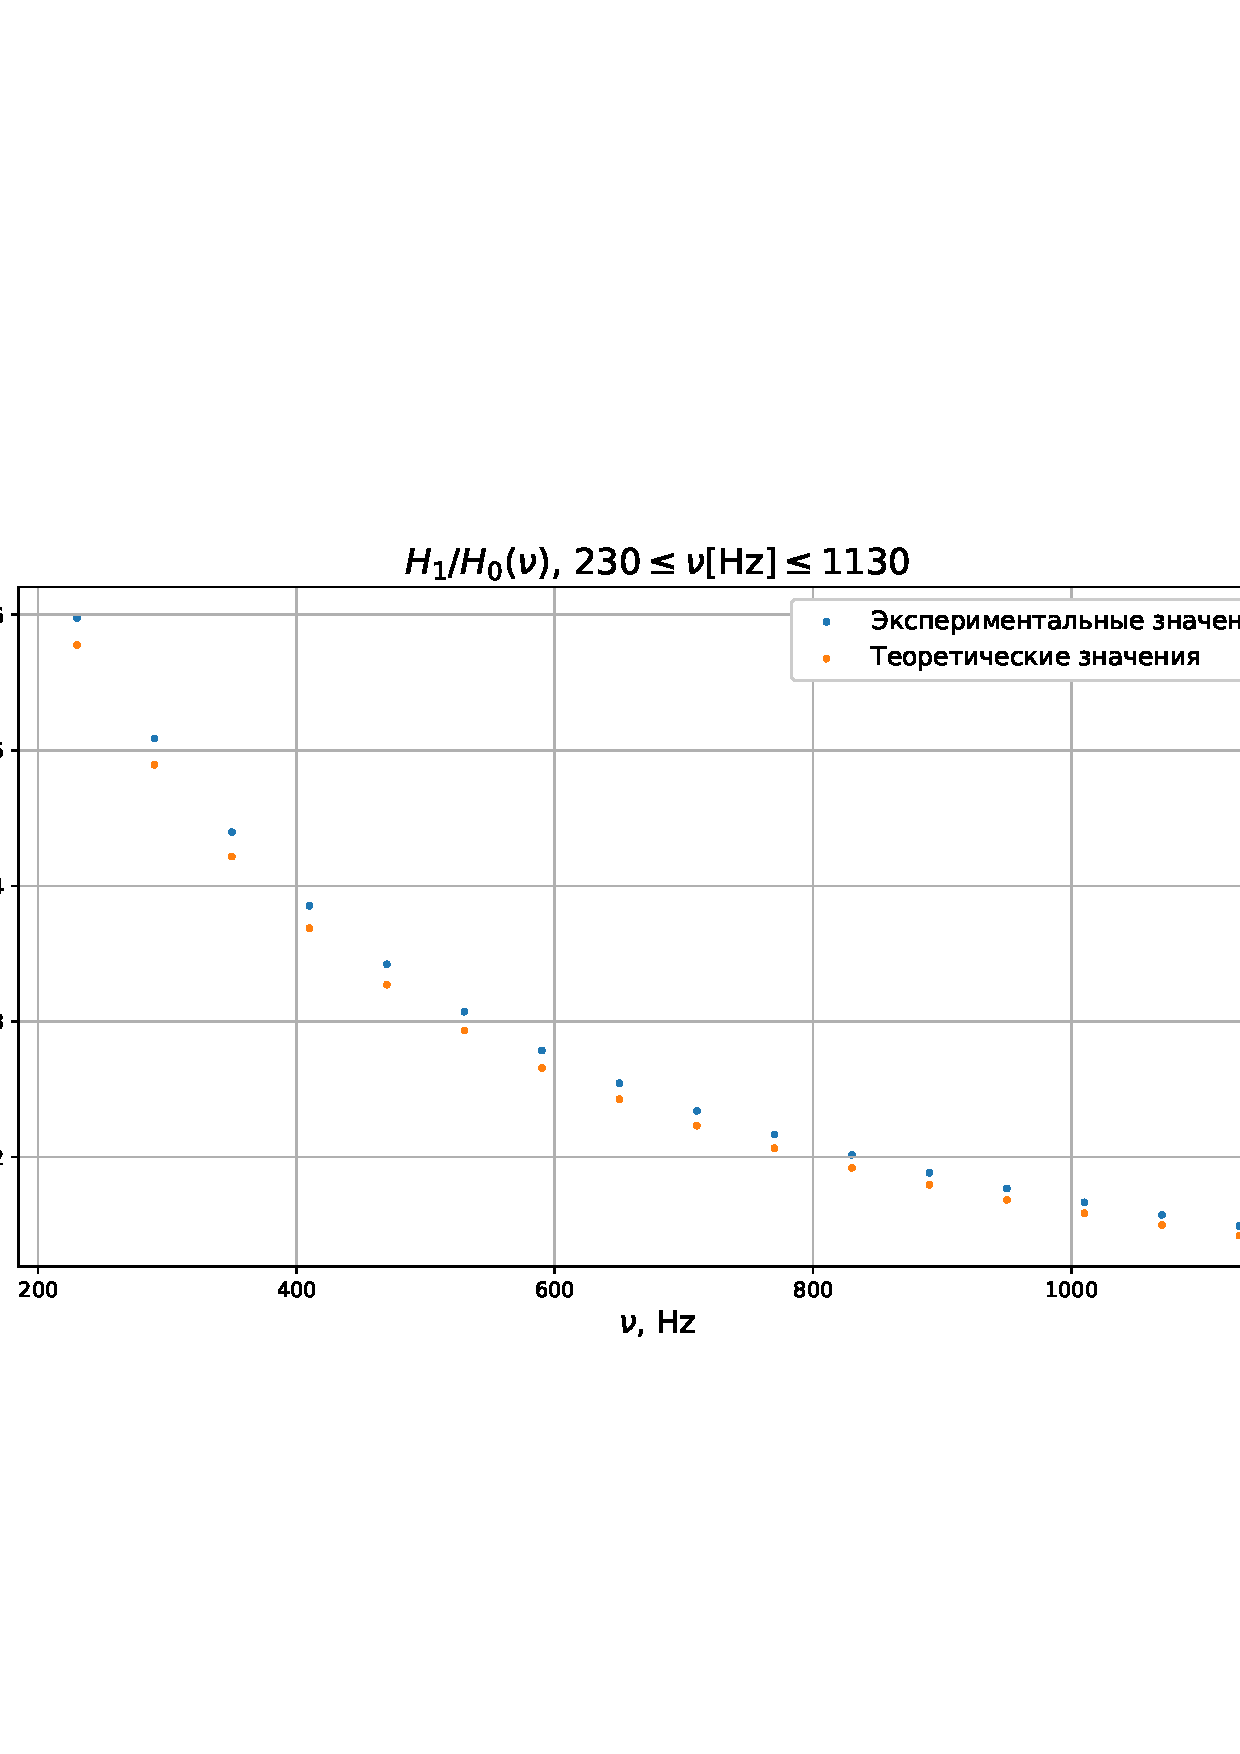
\includegraphics[width=\textwidth]{mid_freq_ratio}}
    \caption{Отношение полей - среднечастотный диапазон}\label{fig:mid_freq_ratio}
    \center{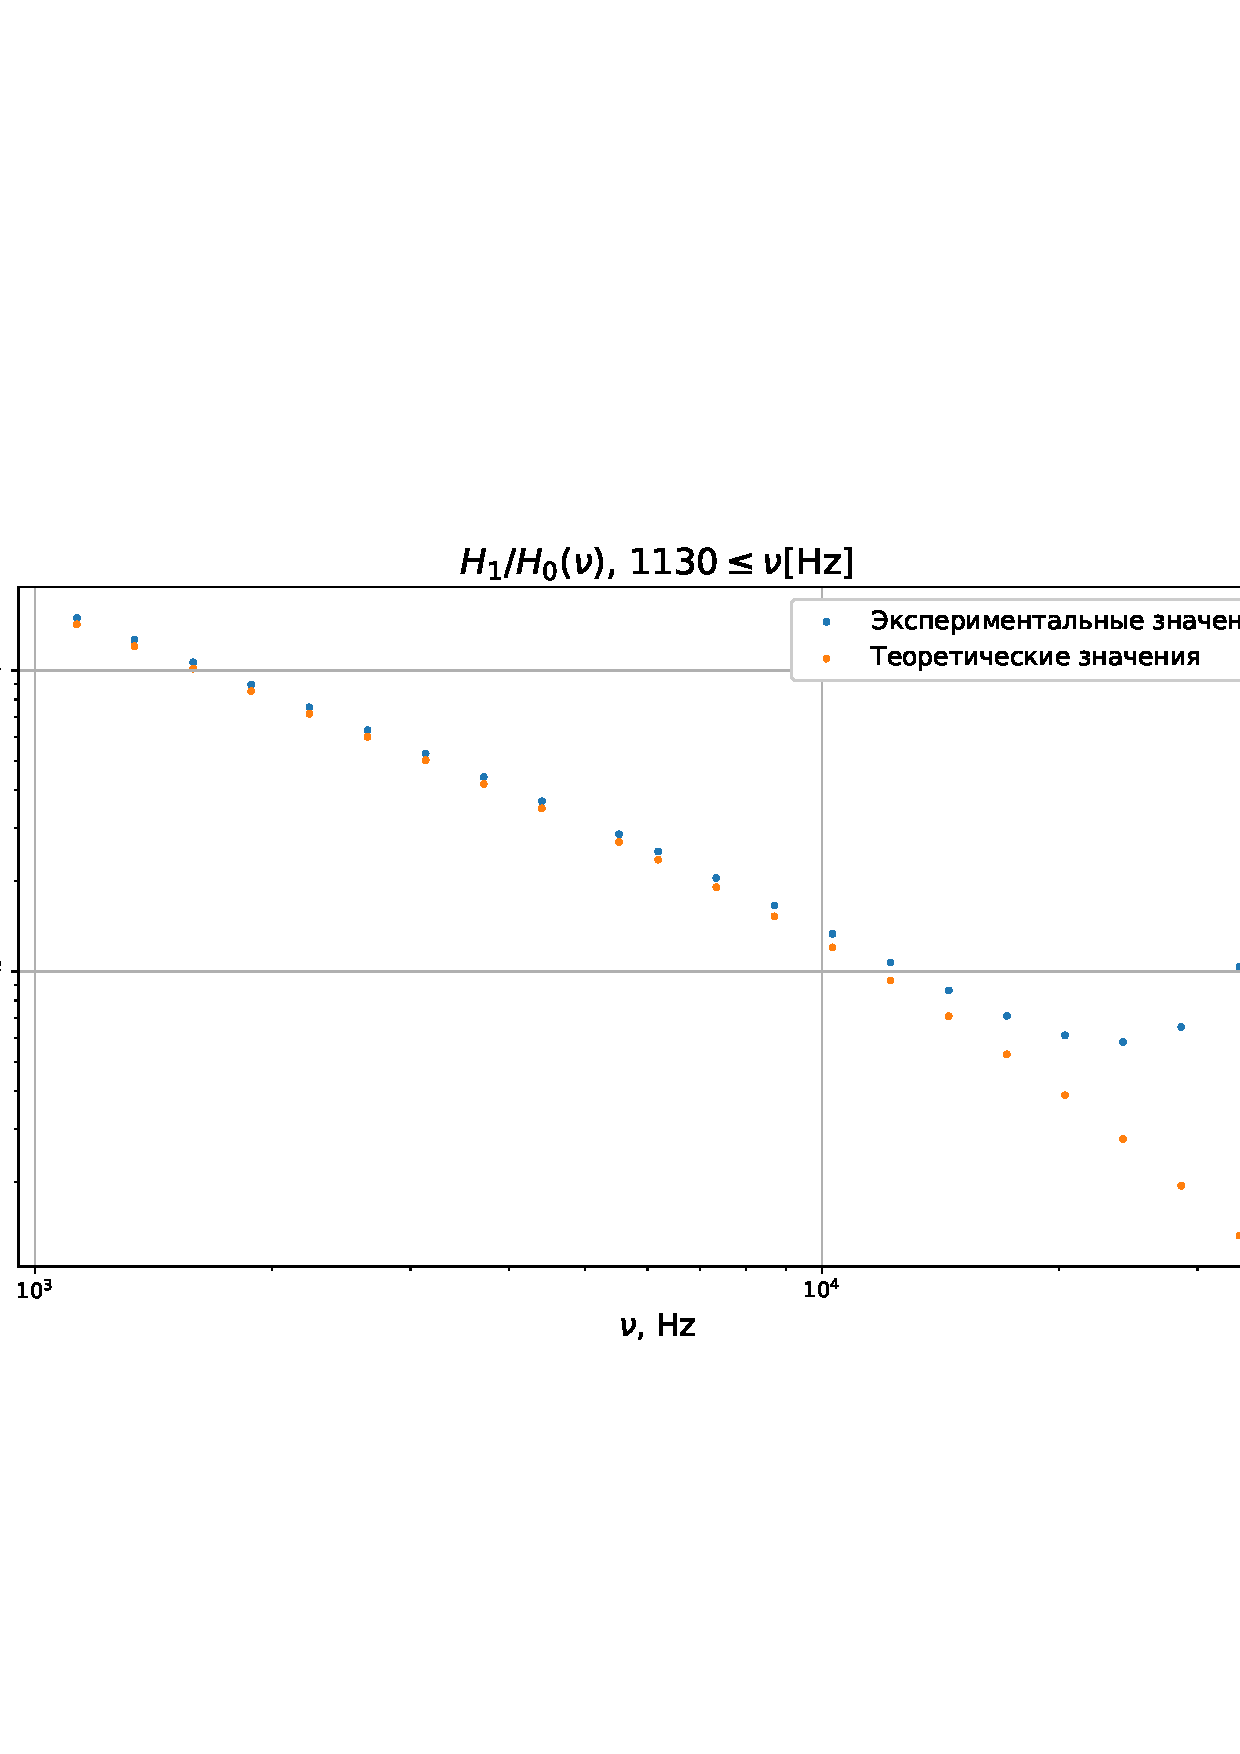
\includegraphics[width=\textwidth]{high_freq_ratio}}
    \caption{Отношение полей - высокочастотный диапазон}\label{fig:high_freq_ratio}
    \newpage
\end{figure}

\section{Вывод}
Мы измерили проводимость материала цилиндра 4 разными способами. Сравним эти данные
между собой

\begin{table}[!h]
\begin{center}
\begin{tabular}{lrrr}
Метод измерения & $\sigma, 10^{7} См/м$ & $\Delta\sigma, 10^{7} См/м$ & $\varepsilon_{\sigma}$\\
\toprule
Отношение амплитуд & 4.4122 & 0.0061 & 0.14\%\\
Разности фаз (низкие частоты) & 4.66 & 0.17 & 3.6\%\\
Разности фаз (высокие частоты) & 4.28 & 0.33 & 7.7\%\\
Индуктивность & 4.49 & 0.07 & 1.6\%\\

\end{tabular}
\end{center}
    \caption{Сравнение результатов различных методов}\label{}
\end{table}

Для данной марки меди проводимость состовляет $\sigma_{точн.} = 5.62\cdot10^{7} См/м$.
Учитывая высокую точность измерения первым методом, предположительно значеня не совпадают
из за неприменимости формул для коэффициентов в нашем случае, в частности из за
приближения о бесконечности цилиндра.

Самым неточным оказался метод измерения через разность фаз при высоких частотах. Это
связано не только с погрешностями измерения разности фаз, но так же с другими эффектами,
которые наблюдаются на графике~\ref{fig:L_nu}. Как видим, при частотах $\sim 5кГц$
зависимость индуктивности не описывается теорией (скорее всего из за токов
Фуко), следовательно, при этих частотах не должна работать и остальная теория.
Как результат, зависимость разности фаз от корня частоты уже не описывается линейной
зависимостью.

Погрешность измерения проводимости через разность фаз при низких частотах в основном
связана с погрешностью измерения самой разности фаз, т.к. погрешность последней
возрастает в несколько раз при подсчете тангенса угла.

Несоответствие величин $\eta = \abs{H_1}/\abs{H_0}$ возможно является следствием ошибки
коэффициента $c$. Чтобы понять это, построим график зависимости $\eta_{эксп}/\eta_{теор}$
от частоты $\nu$

\begin{figure}[h]
    \center{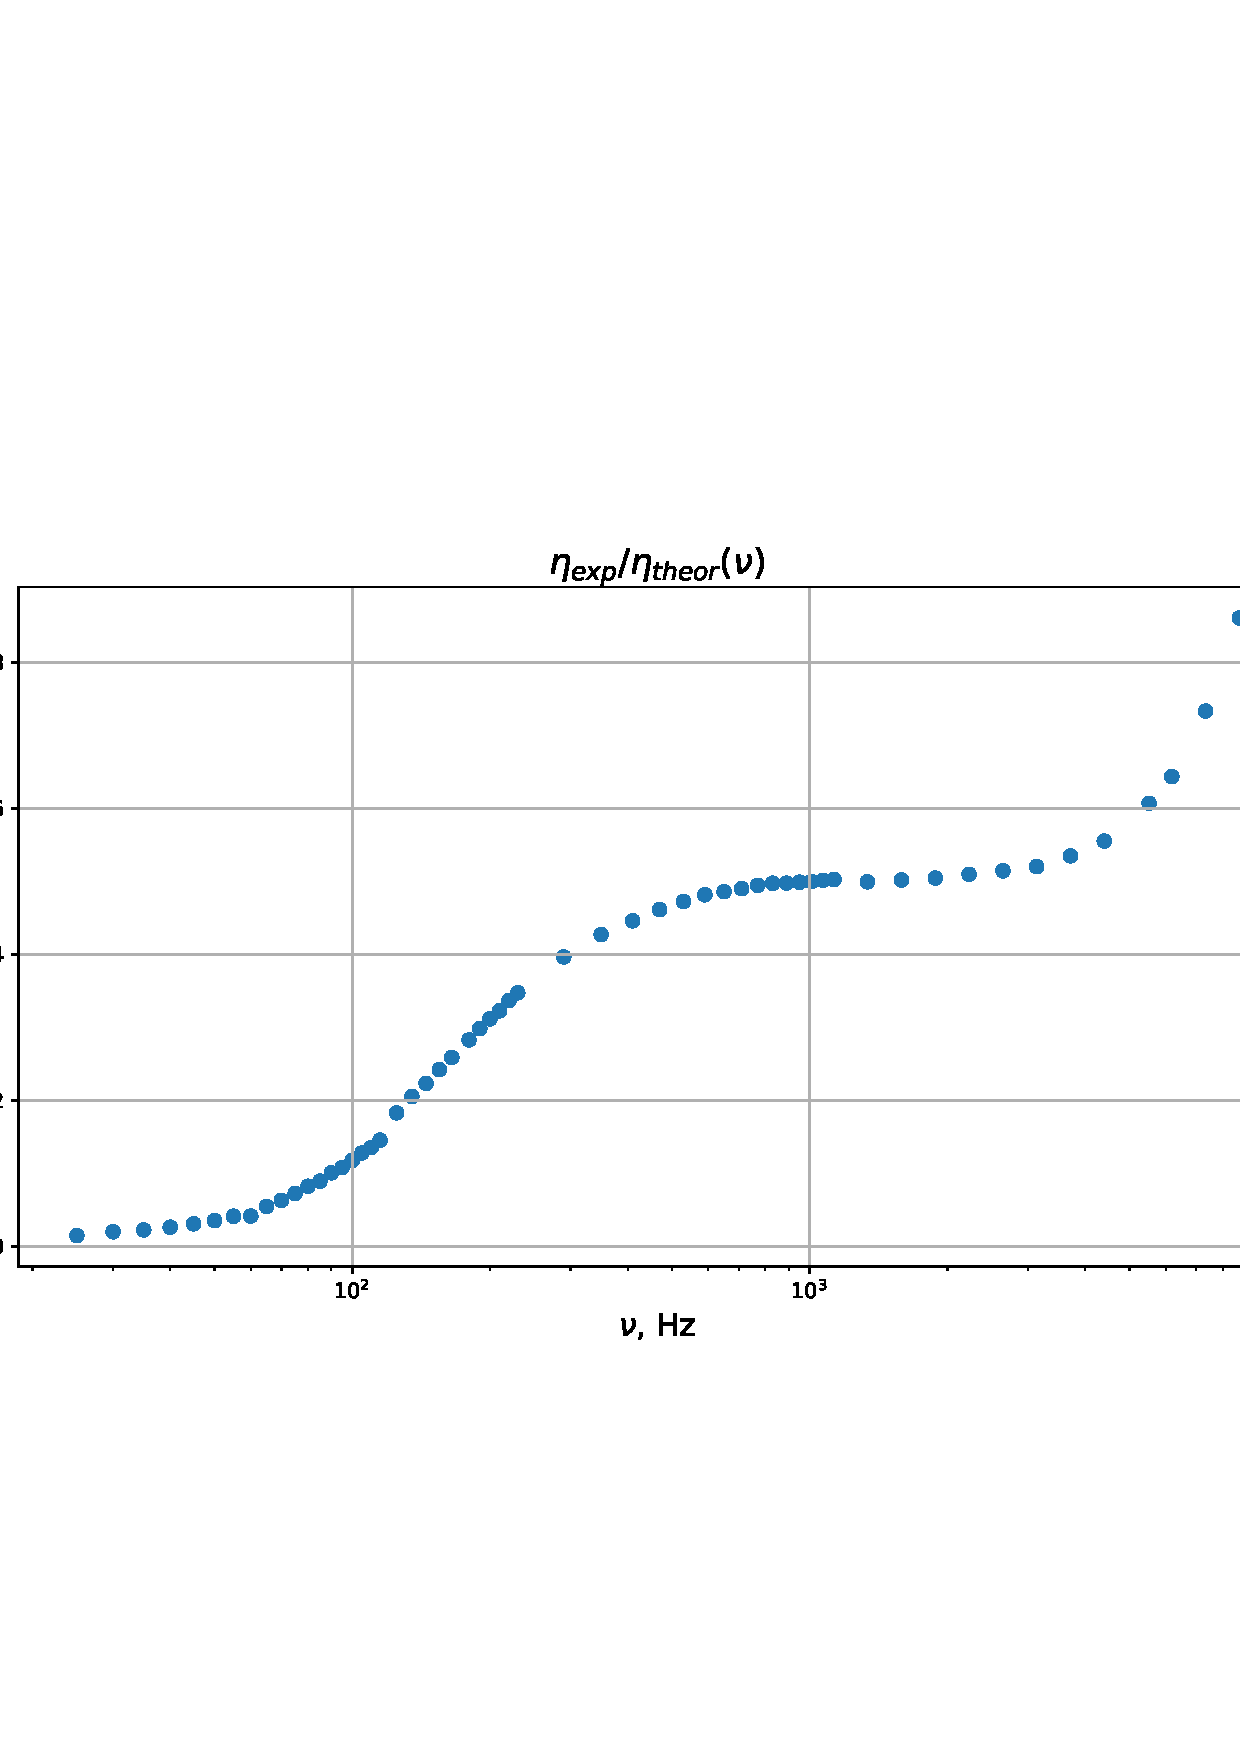
\includegraphics[width=\textwidth]{reduction_ratio}}
    \caption{График зависимости $\eta_{эксп}/\eta_{теор} (\nu)$}
    \label{fig:reduction_ratio}
    \newpage
\end{figure}

Как видим, теория всегда предсказывает большее ослабление, и при том отношение
предсказывании монотонно растет, что свидетельствует о том, что причиной несоответствия
является не ошибка коэффициента $c$, а несоответствие теоретической модели с
действительностью.
\end{document}

